%%%%%%%%%%%%%%%%%%%%%%%%%%%%%%%%%%%%%%%%%%%%%%%%%%%%%%%%%%
\documentclass[xcolor=pdftex,dvipsnames,table,10pt]{beamer}
%handout, if no \pause

\usepackage{tabularx}
\usepackage[]{algorithm2e}
\usepackage{listings}
\usepackage{lstautogobble}
\usepackage{graphicx}
\usepackage{hyperref}
\usepackage{amsmath}
\usepackage{xcolor}
\usepackage{subfigure}
\usepackage[style=authoryear,backend=biber,mincitenames=1,maxcitenames=2, uniquelist=false]{biblatex}
\bibliography{fossilDating.bib}

\newcommand{\Mstrict}{{M1}}
\newcommand{\Mrelaxed}{{M8}}


%\documentclass[handout,xcolor=pdftex,dvipsnames,table]{beamer} % USE THIS WITH pdfpages STUFF
%\usepackage{pgfpages}
%\pgfpagesuselayout{resize to}[a4paper, landscape]

\definecolor{headerColour}{RGB}{180, 230, 245}
\definecolor{headerTitleColour}{RGB}{0, 60, 80}
\definecolor{sectionShadedColour}{RGB}{50, 110, 130}
\definecolor{subsectionHighlightColour}{RGB}{50, 50, 50}
\definecolor{subsectionShadedColour}{RGB}{100, 100, 100}

\setbeamercolor{subsection in sidebar}{fg=subsectionHighlightColour}
\setbeamercolor{subsection in sidebar shaded}{fg=subsectionShadedColour}
\setbeamercolor{structure}{fg=headerTitleColour, bg=headerColour}
\setbeamercolor{title}{fg=headerTitleColour, bg=white}
\setbeamercolor{section in sidebar shaded}{fg=sectionShadedColour}

\usetheme{Goettingen}
\makeatletter\setbeamertemplate{sidebar canvas \beamer@sidebarside}[vertical shading][top=headerColour,bottom=white]\makeatother

%% to suppress subsections in sidebar:
%\setbeamertemplate{subsection in sidebar shaded}
%{\vspace*{-\baselineskip}}
%\setbeamertemplate{subsubsection in sidebar shaded}
%{\vspace*{-\baselineskip}}

\usepackage{amsmath, amssymb}
\usepackage{fancyvrb}


% Font modification
\usefonttheme{professionalfonts}
\usepackage{cmbright}
\usepackage{eulervm}
\newfont{\Ss}{cmcsc12 scaled 1600}

% no navigation symbols at the bottom of frames
\beamertemplatenavigationsymbolsempty
\setbeamertemplate{footline}[frame number] 

\usepackage{multirow} % allows entries across multipe rows in tables
\usepackage{booktabs} % makes fancier rulers in tables
%\usepackage{setspace} % spacing between lines

%%%%%%%%%%%%%%%%%%
%% Bibliography related stuff:
% control space between lines
  \let\oldthebibliography=\thebibliography
  \let\endoldthebibliography=\endthebibliography
  \renewenvironment{thebibliography}[1]{
    \begin{oldthebibliography}{#1}
      \setlength{\parskip}{-0.5ex}
      \setlength{\itemsep}{-0.5ex}
  }{ \end{oldthebibliography} }
% Force entry to be in one line
\setbeamertemplate{bibliography entry title}{}
\setbeamertemplate{bibliography entry location}{}
\setbeamertemplate{bibliography entry note}{}
% Set bullet point shape:
\setbeamertemplate{bibliography item}{-}
%%%%%%%%%%%%%%


\newenvironment{items}{\begin{list}{$\bullet$}{\itemsep0ex plus 0.2ex
\parsep0ex plus 0.2ex \topsep0ex \parskip0ex}}{\end{list}}
\newcommand{\head}[1]
{\slide{\begin{center}\textbf{#1}\vspace*{-0.5\baselineskip}
{\color{red}\rule{\textwidth}{1mm}}\end{center}}}
\parskip0.3ex

\newcommand{\cT}{{\mathcal T}}


%\defbeamertemplate*{title page}{customized}[1][]
%{
%  \titlepage
%  \usebeamerfont{title}\inserttitle\par
%  \usebeamerfont{subtitle}\usebeamercolor[fg]{subtitle}\insertsubtitle\par
%  \bigskip
%  \usebeamerfont{author}\insertauthor\par
%  \usebeamerfont{institute}\insertinstitute\par
%  \usebeamerfont{date}\insertdate\par
%  \usebeamercolor[fg]{titlegraphic}\inserttitlegraphic
%}


\title[Total-evidence dating]{`Total-evidence' Bayesian estimation of phylogeny, divergence times and fossil ages}
\author[]{Alexei Drummond, alexei@cs.auckland.ac.nz}
\date{The Royal Society, London \\ 9th November 2015}
\institute{Professor of Computational Biology \\ Department of Computer Science \\ University of Auckland}
%\titlegraphic{\hspace*{8cm}\includegraphics[height=1.5cm]{figures/cEvo_logo_transparent.png}}
%{\small Link to Script\&Slides:  \url{http://www.tb.ethz.ch/education} 
%}

%%%%%%%%%%%%%% Figure caption setup
\usepackage[compatibility=false]{caption}
\captionsetup[figure]{labelsep=space,justification=centering}
\renewcommand{\figurename}{\scriptsize Figure adapted from}

% syntax: \figureCaption{Citation caption}{Second (real) caption}
% second caption can be skipped, first one has to be suppressed if you want to skip it
\newcommand\figureCaption[2]{%
  \captionsetup{aboveskip=0.1cm,belowskip=0cm}
  \caption{\scriptsize #1}
  \caption*{#2}
}

%%%%%%%%%%%%%% Fixme and comment setup�
\definecolor{red}{HTML}{C92D39}
\definecolor{green}{HTML}{498A44}

% syntax: \fixme{What needs to be fixed}
\newcommand{\fixme}[1]{\textcolor{red}{\texttt{{\bf FIX ME:} #1}}}
% Hide all fixmes by switching the line above to this:
%\newcommand{\fixme}[1]{}

% syntax: \comment{Name of commenter}{C omment}
\newcommand{\comment}[2]{\textcolor{green}{{\bf Comment by {#1}}: #2}}
% Hide all comments by switching the line above to this:
%\newcommand{\comment}[2]{}

\begin{document}

%Slide1
\frame{\titlepage}

\section{Fossilized birth-death process}

\begin{frame}
\frametitle{The fossilized birth-death process}

\end{frame}

\section{Penguin dating}

\begin{frame}
\begin{figure}
\includegraphics[width=0.7\textwidth]{../ag_morpho_data/figures/sa.pdf}
\label{saPostPr}
\end{figure}
\small{Probabilities of each fossil to be a sampled ancestor across models.

{\it P} stands for the partitioned model, {\it G} for gamma variation across sites, {\it Mkv} for conditioning on 
variable characters, {\it R} for relaxed clock model, {\it dns} for $d$, $\nu$, and $s$ tree prior parameterisation, {\it lmp} for $
\lambda$, $\mu$, and $\psi$ tree prior parameterisation.} 
\end{frame}

\begin{frame}
\begin{figure}
\includegraphics[width=\textwidth]{../ag_morpho_data/figures/pp.pdf}
\label{postPredictive}
\end{figure}
\small{The posterior and posterior predictive distributions for (left) tree length, $T$, and genealogical $D_F$ statistics and (right) $B_1$ tree imbalance statistic and Colless's tree imbalance index, $I_c$, for model 8. 

The posterior trees are on the unbalanced end of the predictive distribution.}
\end{frame}

\begin{frame}
\begin{figure}
\includegraphics[width=\textwidth]{../ag_morpho_data/figures/tree.pdf}
\label{penguinTree}
\end{figure}
\footnotesize{A maximum sampled ancestor clade credibility tree for the total-evidence analysis. % with mean node ages. 
The numbers in blue show the posterior supports of clades. The filled red and black circles represent sampled 
ancestors. Fossils with positive evidence of being sampled ancestors are shown in red.}

\end{frame}

\begin{frame}
\begin{figure}
\begin{center}
\includegraphics[width=0.75\textwidth]{../ag_morpho_data/figures/BayesFactors.pdf}
\label{fig:BF}
\end{center}
\end{figure}
\small{The evidence fossil sampled ancestors. The samples above the shaded area have positive evidence to be sampled ancestors and below the shaded area have positive evidence to be terminal nodes.}

\end{frame}

\begin{frame}
\begin{figure}
\includegraphics[width=0.95\textwidth]{../ag_morpho_data/figures/extant_tree.pdf}
\label{fig:divDates}
\end{figure}
\small{The posterior summary tree of extant penguins with 95\% HPD intervals and
posterior supports of clades after removing fossils.}
\end{frame}

\begin{frame}
\begin{figure}
\begin{center}
\includegraphics[width=0.75\textwidth]{../ag_morpho_data/figures/root_ages.pdf}
\label{fig:rootAges}
\end{center}
\end{figure}
\small{The age of root of extant penguins across models including total-evidence analysis under relaxed (8+DNA R) and strict (8+DND S) molecular clocks and 
total-evidence analysis with crown fossils only.}
\end{frame}

\begin{frame}
\frametitle{Dating the evolutionary history of penguins}
\begin{figure}
\includegraphics[width=\textwidth]{penguinTree.pdf}
\end{figure}
\end{frame}

\section{Fossil dating}

\begin{frame}
\begin{figure}
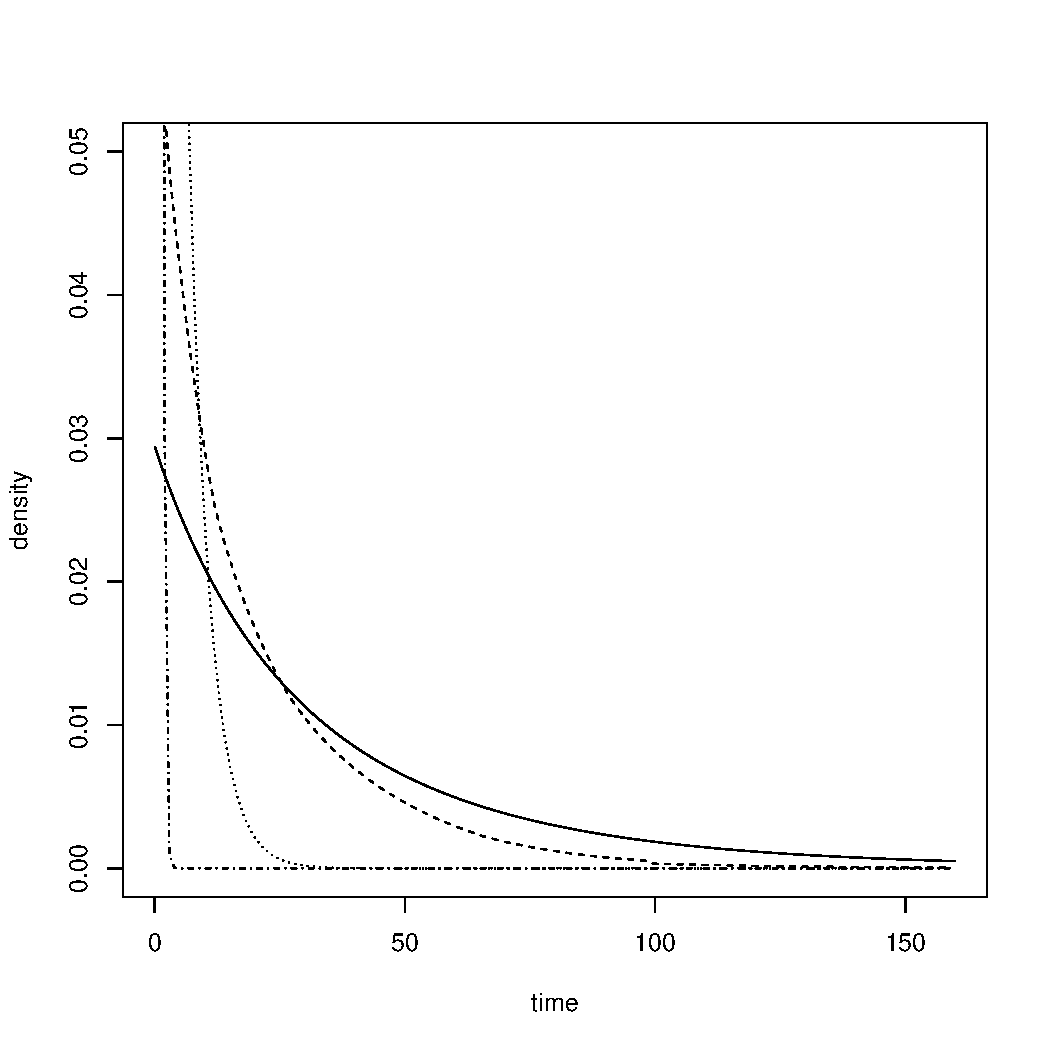
\includegraphics[width=0.6\textwidth]{priors.pdf}
\label{Fig:Prior}
\end{figure}

Density for sampling times under fossilized birth-death process. Dot-dashed line uses priors from \textcite{gavryushkina2015bayesian}. 
Solid line is new prior with implicit assumptions on $T$ and $s$, dashed line results from only assuming implicit prior on $T$,  dotted line results from only assuming implicit prior on $s$.
\end{frame}

\begin{frame}
\begin{figure}
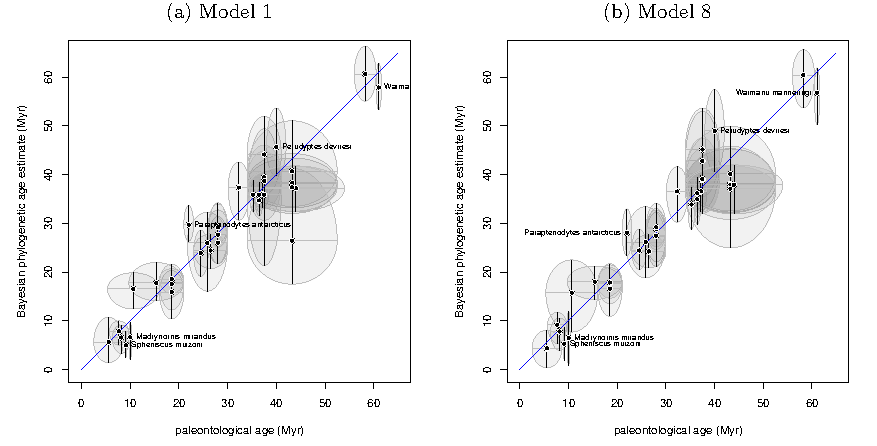
\includegraphics[width=\textwidth]{Figure1.pdf}
\end{figure}
Bayesian phylogenetic age estimates for each of 36 penguin fossils plotted against their palaeontological age estimates, under two alternative evolutionary models. 
The blue line shows the $x=y$. If the vertical line doesn't cross $x=y$, then the midpoint of the geological range is not in the phylogenetic 95\% HPD. 
\end{frame}

\begin{frame}
\begin{figure}
\includegraphics[width=\textwidth]{8_penguins_eNprior/8_fossilDatingHist_younger_wide.pdf}
\end{figure}
Marginal posterior density plots for the phylogenetic age estimate of each of the 18 penguin fossils younger than 30 Myr using \Mrelaxed{}. Red boxes are the superimposed age ranges derived from geological data.
\end{frame}

\begin{frame}
\begin{figure}
\includegraphics[width=\textwidth]{8_penguins_eNprior/8_fossilDatingHist_older_wide.pdf}
\end{figure}
Marginal posterior density plots for the phylogenetic age estimate of each of the 18 penguin fossils older than 30 Myr using \Mrelaxed{}. Red boxes are the superimposed age ranges derived from geological data.
\end{frame}

\begin{frame}
\begin{figure}
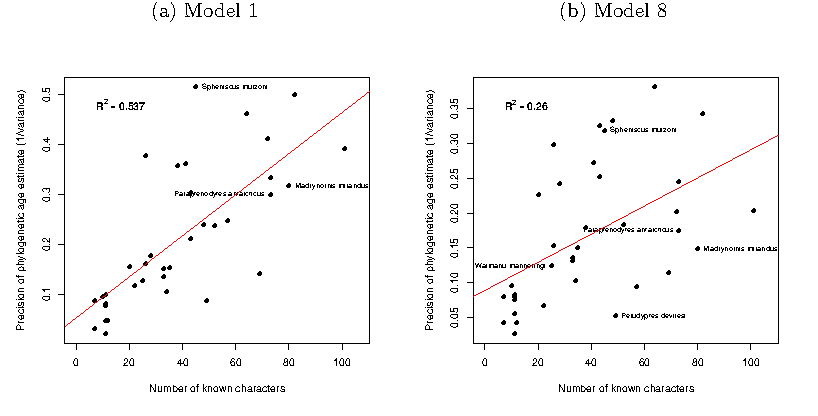
\includegraphics[width=\textwidth]{Figure2.pdf}
\end{figure}
A plot of the number of non-ambiguous morphological sites for the taxon against the precision of the phylogenetic age for (a) \Mstrict{} and (b) \Mrelaxed{} (i.e. the precision is 1/variance in the marginal posterior distribution of the age).
\end{frame}

\begin{frame}
\frametitle{Comparison of age \& BF estimates between models}
\begin{figure}%
\centering
\subfigure[Estimated phylogenetic age of \Mstrict{} against \Mrelaxed{}.]{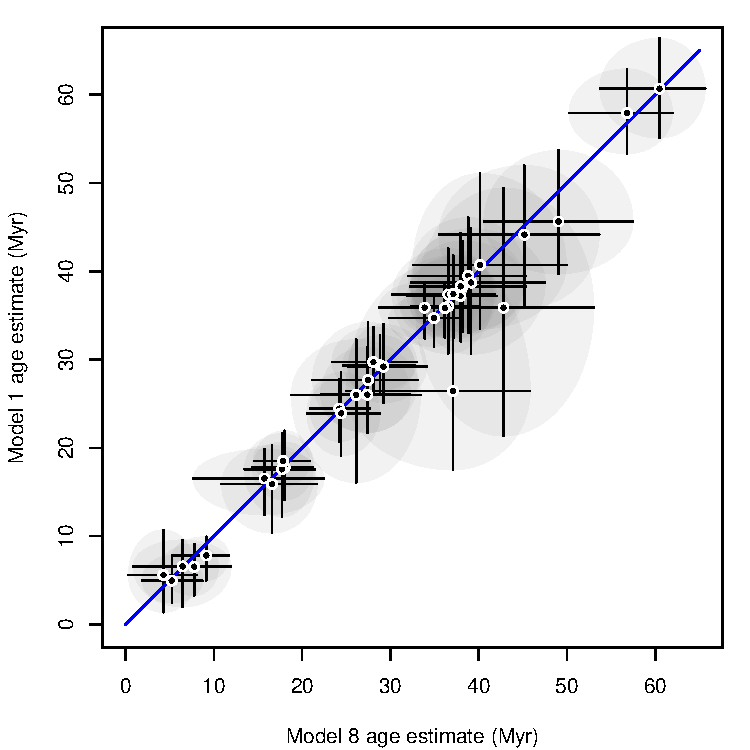
\includegraphics[width=0.45\textwidth]{compareAgeM1M8.pdf}}\qquad
\subfigure[Regression of Bayes factor (BF) for palaeontological range of \Mstrict{} against \Mrelaxed{}.]{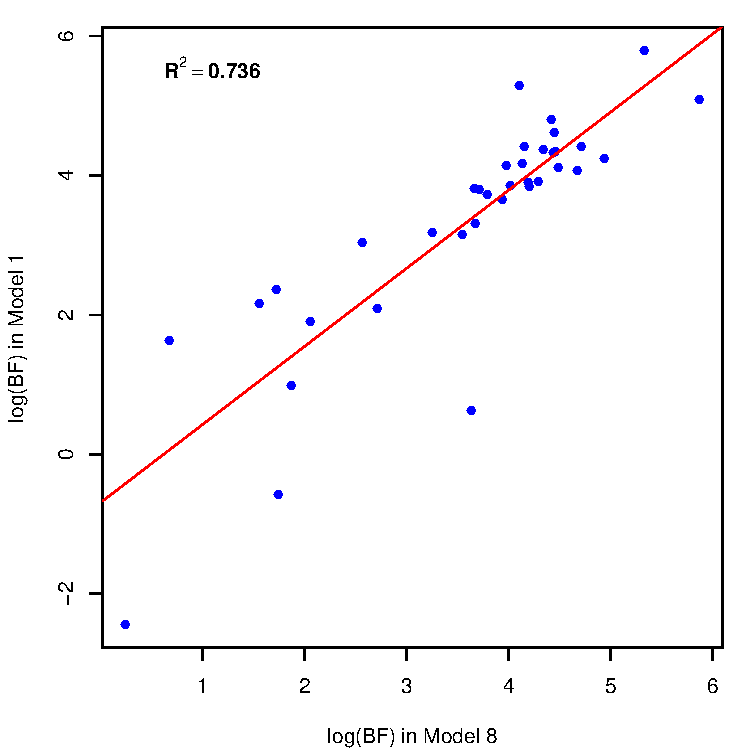
\includegraphics[width=0.45\textwidth]{compareBFM1M8.pdf}}\\
\label{fig:compareM1M8ab}
\end{figure}
\end{frame}

\begin{frame}
\frametitle{Comparison of probability \& error between models}
\begin{figure}%
\centering
\subfigure[Regression of posterior probability of palaeontological range of \Mstrict{} against \Mrelaxed{}.]{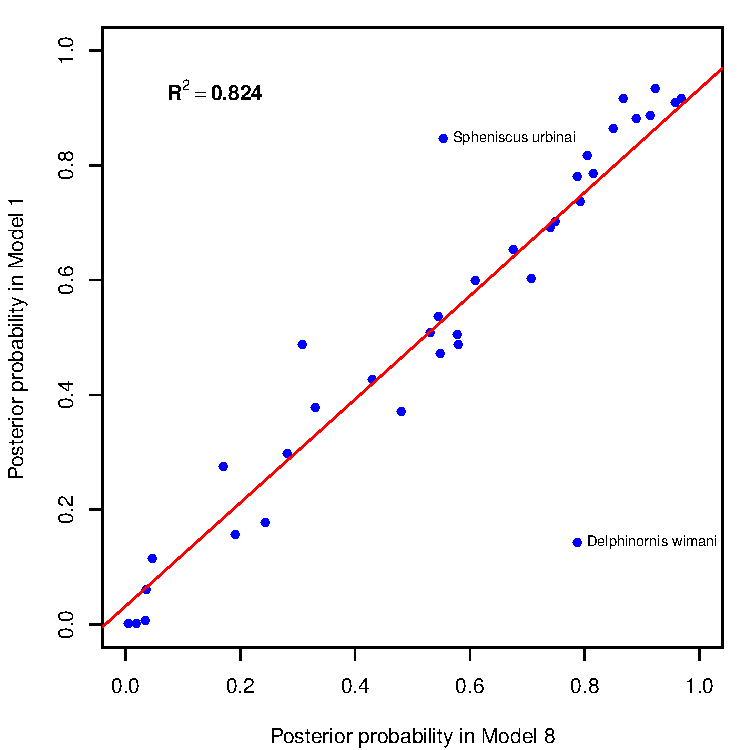
\includegraphics[width=0.45\textwidth]{comparePostM1M8.pdf}}\qquad
\subfigure[Regression of error in estimated phylogenetic age of \Mstrict{} against \Mrelaxed{}.]{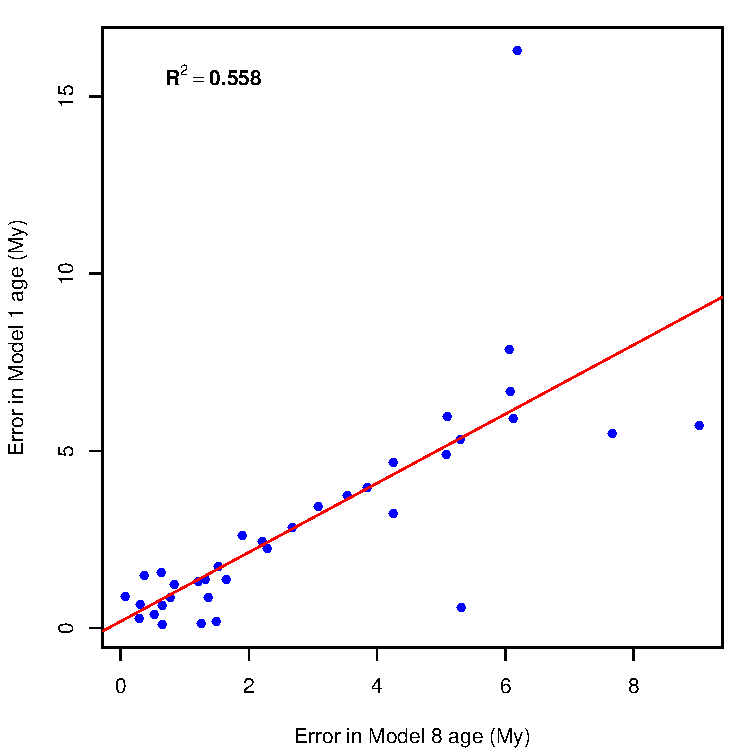
\includegraphics[width=0.45\textwidth]{compareErrorM1M8.pdf}}\\
\label{fig:compareM1M8cd}
\end{figure}
\end{frame}


\end{document}
